\chapter{Extension of LTC to n Dimension And Implementation}

\TG{A transition with the previous chapter is really missing, here or in the conclusion
of the previous chapter. You also need to explain why you are doing this:
why do we need a multi-dimensional implementation, why you chose LTC, etc}

In this section we give the notation of LTC and provide a norm-independent
formulation of LTC in dimension $n$. By $n$ we refer to the dimension of the
data points $x_i$. To handle time, LTC actually operates in dimension $n+1$. And
we present how LTC n-dimensions is implemented. Our code is available at
\url{https://github.com/big-data-lab-team/stream-summarization} under MIT
license.

\section{Preliminary comments}

We note that the formulation of LTC 
in~\cite{schoellhammer2004lightweight} relies on the intersection of 
\emph{convex cones} in dimension $n+1$. For $n=1$, it corresponds to 
the intersection of triangles, which can efficiently be computed by 
maintaining boundary lines, as detailed previously. In higher 
dimension, however, cone intersections are not so straightforward, due 
to the fact that the intersection between cones may not be a cone.

To address this issue, we formulate LTC as an intersection test between
\emph{balls} of dimension $n$, that is, segments for $n=1$, disks for
$n=2$, etc. Balls are defined from the \emph{norm} used in
the vector space of data points. For $n=1$, the choice of the norm does
not really matter, as all p-norms and the infinity norm are identical.
In dimension $n$, however, norm selection will be critical.

\section{Algebraic formulation of LTC}

\subsection{Definitions}

Let $(u_0^k, y_0^k) \in \mathbb{R}^{n+1}$ be the latest transmitted point. For convenience, all the subsequent points will be
expressed in the orthogonal space with origin $(\tau_k, \xi_k)$. We denote by $(v_j, z_j)_{j \in \llbracket 0, m \rrbracket}$ such points:
\begin{equation*}
\forall j \leq m,\  (v_j, z_j) = (u_j^k - \tau_k, y_j^k - \xi_k)
\end{equation*}
Let $\mathcal{B}_j$ be the ball of $\mathbb{R}^n$ of centre $\frac{v_1}{v_j}z_j$ and radius
$\frac{v_1}{v_j}\epsilon$:
\begin{equation*}
\mathcal{B}_j = \left\{ z \in \mathbb{R}^n,\\norm{z-\frac{v_1}{v_j}z_j} \leq\frac{v_1}{v_j}\epsilon \right\}
\end{equation*}
Note that $v_1$ is defined as soon as one point is received after the last
transmission.

\subsection{LTC property}

We define the \emph{LTC property} as follows:
\begin{equation*}
\exists z \in \mathbb{R}^n, \ \forall j \in \llbracket 1, m \rrbracket, \norm{\frac{v_j}{v_1}z-z_j} \leq
\epsilon.
\end{equation*}
The original LTC algorithm ensures that the LTC property is
verified between each transmission. Indeed, all the data points
$z$ such that $(v_1, z)$ is between the high line and the low line
verify the property. Line 13 in Algorithm~\ref{algo:ltc} guarantees that
such a point exists.

The LTC property can be re-written as follows:
\begin{equation*}
\exists z \in \mathbb{R}^n, \ \forall j \in \llbracket 1, m \rrbracket, \norm{z-\frac{v_1}{v_j}z_j} \leq
\frac{v_1}{v_j}\epsilon
\end{equation*}
that is:
\begin{equation}
\bigcap_{j=1}^m \mathcal{B}_j \neq \O
\label{eq:ltc-property}
\end{equation}
Note that $(\mathcal{B}_j)_{j \in \llbracket 1, m \rrbracket}$ is a sequence
of balls of strictly decreasing radius, since $v_j > v_1$.

\section{Algorithm}

The LTC algorithm generalized to dimension $n$ tests that the LTC 
property in Equation~\ref{eq:ltc-property} is verified after each reception of a data 
point. It is written in Algorithm~\ref{algo:general-ltc}.
\begin{algorithm}
\begin{algorithmic}[1]
\Input
   \Desc{$(u^k_j, y^k_j)$}{$\quad \quad $Received data stream}
   \Desc{$\epsilon$}{$\quad \quad$Error bound}
\EndInput
\Output
   \Desc{tr}{Transmitted points}
\EndOutput

\State tr = ($\tau, \xi$) = ($u^0_0, y^0_0$) \Comment{Last transmitted point}
\State k = 0 ; j = 0
\While{True}
    \State j += 1
    \State ($v_j, z_j$) = ($u_j^k - \tau, y_j^k - \xi$)
    \If{$\bigcap_{l=1}^j{\mathcal{B}_l} = \O$}
        \State Pick $z$ in $\bigcap_{l=1}^{j-1}{\mathcal{B}_j}$ \Comment{Transmit point}
        \State tr = ($\tau$, $\xi$) = ($u^k_{j-1}, z$)
        \State k += 1
        \State j = 1
    \EndIf
\EndWhile
\end{algorithmic}
\caption{Generalized LTC.}
\label{algo:general-ltc}
\end{algorithm}

\section{Ball intersections}

Although Algorithm~\ref{algo:general-ltc} looks simple, one should not
overlook the fact that there is no good general algorithm to test
whether a set of balls intersect. The best general algorithm we could find
so far relies on Helly's theorem which is formulated as follows~\cite{helly1923mengen}:
\begin{theorem}
Let $\left\{ X_i \right\}_{i \in \llbracket 1, m \rrbracket}$ be a collection of convex subsets of $\mathbb{R}^n$. If the intersection of every $n+1$
subsets is non-empty, then the whole collection has an non-empty intersection.
\end{theorem}
\noindent This theorem leads to an algorithm of complexity ${m \choose n+1}$ which is not usable in resource-constrained environments.

The only feasible algorithm that we found is norm-specific. It
maintains a representation of the intersection
$\bigcap_{j=1}^{m}{\mathcal{B}_j}$ which is updated at every iteration.
The intersection tests can then be done in constant time. However,
updating the representation of the intersection may be costly
depending on the norm used. For the infinity norm, the representation
is a rectangular cuboid which is straightforward to update by
intersection with an n-ball.
For the Euclidean norm, the representation is a volume with no particular property,
which is more costly to maintain.

\section{Effect of the norm}

As mentioned before, norm selection in $\mathbb{R}^n$ has a critical
impact on the compression error and ratio. To appreciate this effect,
let us compare the infinity norm and the
Euclidean norm in dimension 2. By comparing the unit disk to a
square of side 2, we obtain that the compression ratio of a random stream would
be $\frac{4}{\pi}$ times larger with the infinity norm than with the 
Euclidean norm. In 3D, this ratio would be $\frac{6}{\pi}$. Conversely, 
a compression error bounded by $\epsilon$ with the infinity norm 
corresponds to a compression error of $\frac{\epsilon}{\sqrt{n}}$ with 
the Euclidean norm. Unsurprisingly, the
infinity norm is more tolerant than the Euclidean norm.

It should also be noted that using the infinity norm in $\mathbb{R}^n$ 
boils down to the use of the 1D LTC algorithm independently in each 
dimension, since a data point will be transmitted as soon as the linear 
approximation doesn't hold in any of the dimensions. For the Euclidean 
norm, however, the multidimensional and multiple unidimensional 
versions are different: the multiple unidimensional version 
behaves as the infinity norm, but the multidimensional version is more 
stringent, leading to a reduced compression rate and error.

To choose between the multidimensional implementation and multiple 
unidimensional ones, we recommend to check whether the desired 
error bound is expressed independently for every sensor, or as an aggregate error between them.
The multidimensional version is
more appropriate for multidimensional sensors, for instance 3D 
accelerometers or 3D gyroscopes, and the multiple unidimensional 
version is more suitable for multiple independent sensors, for 
instance a temperature and a pressure sensor.
%~ For instance, in case of a 3D accelerometer, if the error 
%~ is expressed simply as 
%~ ``10~mg", then the multidimensional version should be chosen because it 
%~ will guarantee that the norm of the 3D acceleration vector will be 
%~ reconstructed with an error less than 10~mg. Conversely, if the error is 
%~ specified as ``10~mg in x, 
%~ 10~mg in y and 10~mg in z", then the multiple unidimensional version 
%~ should be used.

\section{Implementation of LTC n-dimension}
\label{sec:implementation}
To implement \acrshort{ltc} in n dimensions with the infinity norm, we maintain a cuboid
representation of $\cap_{l=1}^j{\mathcal{B}_l}$ across the iterations of the
\texttt{while} loop in Algorithm~\ref{algo:general-ltc}. The implementation
works with constant memory and requires limited CPU time.

% With the Euclidean norm, the intersection test is more complex. We keep in
% memory a growing set $S$ of n-balls and the bounding box $B$ of their
% intersection. 
With the Euclidean norm, the intersection test is more complex. We keep in
memory a growing set $S$ of n-balls and the bounding box $B$ which represents an
approximate range of their intersection. We define $B$ as follows:
\begin{equation*}
    B = \bigcap_{l=1}^{j-1} box(\mathcal{B}_l) 
\end{equation*}
Where \texttt{box()} is a function that returns the bounding box of an n-ball.
Then, when a new point arrives, we consider the associated n-ball
$\mathcal{B}_j$ and our intersection test works as in
Algorithm~\ref{algo:euclidean}. Firstly, we check the intersection between
box($\mathcal{B}_j$) and $B$ (Algorithm~\ref{algo:euclidean}, line 11). To
restrict memory usage, $B$ only covers a set $S$ of n-balls were the size of $S$
is limited to $L_s$. Secondly, for each $\mathcal{B}_i$ in $S$, we check the
intersection between $\mathcal{B}_i$ and $\mathcal{B}_j$ (line 14). In addition
$\mathcal{B}_i$ will be removed if it includes $\mathcal{B}_j$, because if
$\mathcal{B}_j$ has intersection with n-balls in $S$ then a bigger n-ball which
contains $\mathcal{B}_j$ must also have intersection.
% \english{because smaller n-ball intersects
% $\mathcal{B}_j$ than a bigger n-ball which contains the smaller one (line 17, 18 in
% Algorithm~\ref{algo:euclidean})} \TG{English is not correct}.
Finally, we search a point in intersection of all n-balls in $S$, using plane
sweep~\cite{shamos1976geometric, souvaine2008line} and bisection initialized by
the bounds of $B$. Function \texttt{find\_bisection(S, B)} (see
Algorithm~\ref{algo:find_bisection_function}) and \texttt{recursive(S, L, R, N,
$X^n$)} (see Algorithm~\ref{algo:recursive}) show how it works. 

% describe function find_bisection
In function \texttt{find\_bisection(S, B)}, we selected dimension of n-balls as
$n$ used at the beginning of bisection, also computed minimum/maximum value of
bounding box $B$ at the $n_{th}$ dimension, which corresponds to $left$ and
$right$ in bisection method. The return object $X^n$ represents a n-dimensional
point in the intersection of all n-balls in $S$. It would be returned if we have
$True$ result from function \texttt{recursive(S, L, R, N, $X^n$)}. $X^n$ is
initialized and put into function \texttt{recursive(S, L, R, N, $X^n$)}, because
it is necessary to update the values (see Algorithm~\ref{algo:recursive} line
26) of $X^n$ during the recursive process. In line 27 of
Algorithm~\ref{algo:recursive}, it happens in case of $left > right$, which
means:
\begin{equation*}
    mid \  \bigcap \  (min\_id \cap max\_id) = \text{\O}
\end{equation*}

In Algorithm~\ref{algo:euclidean} line 14 and 15, it is guaranteed that any two
n-balls in $S$ has intersection. Therefore, any point in the intersection of
$min\_id$ and $max\_id$, could be used for determining the direction of
bisection. In our implementation, we select a point in connection of these two
n-ball's center, which also locates in intersecting object (line/chord when
order=2, plane/circle when order=3). Figure~\ref{fig:compare_point} shows the
point we selected in 2D.

%discuss the time complexity
According to our implementation for Euclidean norm, if the $L_s$ is undefined
($L_s$ is infinity), the operations in Algorithm~\ref{algo:euclidean} and
Algorithm~\ref{algo:find_bisection_function} before the function
\texttt{recursive()} need $O(n)$ complexity. In the \texttt{recursive()}
function, the bisection from line 12 to line 32 in
Algorithm~\ref{algo:recursive} needs $O(\log{2\epsilon})$, because the $left$
and $right$ are initialized from the bounding box $B$, where $|left - right|
\leqslant 2\epsilon$. Moreover, computing $left$ and $right$ which used for next
dimension in \texttt{recursive()} function needs $O(n)$. Thereby, when the data
stream is two-dimensional, the time complexity of LTC n-dimension for Euclidean
norm is $O(n) + O(\log{2\epsilon})\times O(n)$ = $O(n \times \log{2\epsilon})$,
where $n$ is the number of the data points we seen so far. In the same way, if
we process 3-dimensional stream with our algorithm with Euclidean norm, it needs
extra $O(n \times \log{2\epsilon})$ time in recursion, the total time complexity
is $O(n) + O(\log{2\epsilon})\times (O(n) + O(\log{2\epsilon})\times O(n))$ =
$O(n\times(\log{2\epsilon})^{2})$. Finally, our implementation for Euclidean
norm gives $O(n\times(\log{2\epsilon})^{d-1})$ time complexity for d-dimensional
data stream.


\begin{figure}
  \centering
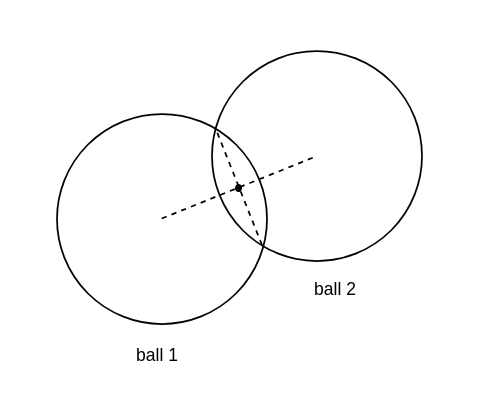
\includegraphics[width=0.7\textwidth]{figures/point-in-chord.png}
\caption{The point selected to determine the direction}
\label{fig:compare_point}
\end{figure}


\begin{algorithm}
\begin{algorithmic}[1]
\Input
    \Desc{$S$}{Set of intersecting n-balls}
    \Desc{$B$}{Bounding box of the intersection of n-balls in $S$}
    \Desc{$\mathcal{B}_j$}{New n-ball to check}
    \Desc{$L_s$}{The maximum length of $S$}
\EndInput
\Output
    \Desc{$S$}{Updated set of intersecting n-balls}
    \Desc{$B$}{Updated bounding box}
    \Desc{$T$}{True if all the n-balls in S and $\mathcal{B}_j$ intersect}
    \Desc{$x$}{Point inside intersection. It might be Null}
\EndOutput

%\If{$\mathcal{B}_j \cap B = \text{\O}$} \Comment{Ball is outside bounding box}
\If{$S$.length $\geqslant L_s \parallel$ box($\mathcal{B}_j$) $\cap B = \text{\O}$} \Comment{N-ball is outside bounding box}
    \State \Return ($S$, $B$, False, Null)
\EndIf
\If{$\exists\ \mathcal{B}_i \in S$ s.t. $\mathcal{B}_j \cap \mathcal{B}_i = \text{\O}$}
    \State \Return ($S$, $B$, False, Null) \Comment{Some n-balls don't intersect}
\EndIf
\If{$\exists\ \mathcal{B}_i \in S$ s.t. $\mathcal{B}_j \subset \mathcal{B}_i$} \Comment{Remove inclusions}
%\State Remove $\mathcal{B}_i$ from $B$. %Add $\mathcal{B}_j$ to $B$. 
    \State Remove $\mathcal{B}_i$ from $S$. %Add $\mathcal{B}_j$ to $S$. 
\EndIf
\State $B$ = box($\mathcal{B}_j$) $\ \bigcap\ $ $B$
\State $S$ = $S \ \bigcup \  \{\mathcal{B}_j\}$
\State $x$ = find\_bisection($S$, $B$) \Comment{This can take some time}
\If{$x$ == Null}
    \State \Return ($S$, $B$, False, Null)
\Else
    \State \Return ($S$, $B$, True, $x$)
\EndIf
\end{algorithmic}
\caption{Intersection test for Euclidean n-balls.}
\label{algo:euclidean}
\end{algorithm}


\begin{algorithm}[H]
\begin{algorithmic}[1]
\Input
    \Desc{$S$}{Set of n-balls}
    \Desc{$B$}{Bounding box of the intersection of n-balls in $S$}
\EndInput
\Output
    \Desc{$X^n$}{N-dimensional point in all n-balls in $S$, $X^n = (x_1,...,x_n)$}
\EndOutput

\State $n$ = dimension of n-balls
\State $left$ = min\_value($B$, $n$) \Comment{Minimum value of $B$ along $n^{th}$ dimension}
\State $right$ = max\_value($B$, $n$) \Comment{Maximum value of $B$ along $n^{th}$ dimension}
\State $X^n$ = Null
\If{recursive(S, left, right, n, $X^n$)}
    \State \Return $X^n$
\Else
    \State \Return Null
\EndIf
\end{algorithmic}
\caption{Function find\_bisection(S, B)}
\label{algo:find_bisection_function}
\end{algorithm}

\begin{algorithm}
\begin{algorithmic}[1]
\Input
   \Desc{$S$}{Set of n-balls}
   \Desc{$L$}{Min value used in bisection}
   \Desc{$R$}{Max value used in bisection}
   \Desc{$N$}{The $N^{th}$ dimension, $N \in \{1...n\}$}
   \Desc{$X^n$}{N-dimensional point which records point of intersection, $X^n$ = $(x_1,...,x_n)$} 
   %\TG{\#\#If you know the point already, what are you looking for?}
\EndInput
\Output
   \Desc{$T$}{True if a point is found by using bisection}
\EndOutput
\If{$N$ == 1}
    \State $X^n.x_N$ = $\frac{L+R}{2}$; $\ $\Return True
\EndIf
\While{$L < R$ }
    \State $mid$ = $\frac{L+R}{2}$; $\ surface$ = $\{x_{N}...x_{n}\}$
    \State $left$ = -$\infty$; $\ right$ = +$\infty$
    \ForAll{$\mathcal{B}_i \in S$}
        \State $min$ = min\_value($\mathcal{B}_i \cap surface$, N-1)
        \State $max$ = max\_value($\mathcal{B}_i \cap surface$, N-1)
        \If{$left < min$}
            \State $left$ = $min$; $\ min\_id$ = $\mathcal{B}_i$
        \EndIf
        \If{$right > max$}
            \State $right$ = $max$; $\ max\_id$ = $\mathcal{B}_i$
        \EndIf
    \EndFor
    
    \If{$left \leqslant right$}
        \State $X^n.x_N$ = $mid$; $\ $
        \Return recursive($S$, $left$, $right$, $N-1$, $X^n$)
    \ElsIf{$\ \forall\ P$ (Point) $\in (min\_id \cap max\_id)$ s.t. $P.x_N < mid$}
        \State $R$ = $mid$
    \Else
        \State $L$ = $mid$
    \EndIf
\EndWhile
\State \Return False
\end{algorithmic}
\caption{Function recursive(S, L, R, N, $X^n$)}
\label{algo:recursive}
\end{algorithm}


%% conclusion
\section{Conclusion}
In this chapter, we give a notation for the original \acrshort{ltc} algorithm
and a pseudo-code with our notation and definitions. To generalize
\acrshort{ltc} to dimension $n$, the \acrshort{ltc} property has been re-written
in Section~\ref{sec:ltc-property}. According to Section~\ref{sec:effect-norm},
we have known that the n-dimensional \acrshort{ltc} might get different results
in different norms. In the Euclidean norm, it is more difficult to check the
intersection and record this inter section in memory. We introduce the method of
combination of plane sweep and bisection for intersection test in the Euclidean
norm, but it spends more processing time and costs more memory to record a
sequence of n-balls than the method for the Infinity norm. In the next chapter,
we will show the result of using n-dimensional \acrshort{ltc} on the
accelerometer data of human activities. 

